% =====================================================================
%  MEMORIA DEL TFG / TFM
%  Compilar:  make memoria      (o: cd memoria && latexmk main.tex)
%  Rellena primero config/datos.tex.
% =====================================================================
\documentclass[12pt, a4paper, twoside, openright]{book}

% =====================================================================
%  DATOS DEL TRABAJO
%  Es el ÚNICO fichero que hay que editar al empezar. Todo lo demás
%  (portada, metadatos del PDF, presentaciones, nombre de los
%  entregables generados por la CI) se alimenta de estas macros.
% =====================================================================

% --- Tipo de trabajo -------------------------------------------------
\newcommand{\TipoTrabajo}{Trabajo Fin de Grado}      % o: Trabajo Fin de Máster
\newcommand{\TipoCorto}{TFG}                         % o: TFM
\newcommand{\Titulacion}{Grado en Ingeniería en Tecnologías Industriales}

% --- Título (español e inglés) ---------------------------------------
\newcommand{\Titulo}{Título del trabajo en español}
\newcommand{\TituloEN}{Project title in English}

% --- Personas ---------------------------------------------------------
\newcommand{\Autor}{Nombre Apellido1 Apellido2}
\newcommand{\Director}{Nombre Apellido1 Apellido2}
\newcommand{\Codirector}{}                           % dejar vacío si no hay

% --- Institución ------------------------------------------------------
\newcommand{\Universidad}{Universidad Pontificia Comillas}
\newcommand{\Escuela}{Escuela Técnica Superior de Ingeniería (ICAI)}
\newcommand{\LogoUniversidad}{figuras/logo_universidad}

% --- Fechas -----------------------------------------------------------
\newcommand{\Lugar}{Madrid}
\newcommand{\FechaEntrega}{Junio 2027}
\newcommand{\CursoAcademico}{2026-2027}

% --- Palabras clave -----------------------------------------------------
\newcommand{\PalabrasClave}{palabra 1, palabra 2, palabra 3, palabra 4}
\newcommand{\Keywords}{keyword 1, keyword 2, keyword 3, keyword 4}

% --- Entrega ----------------------------------------------------------
% Nombre base de los PDF que publica la CI (sin espacios ni tildes).
% Convención: <TIPO>_<Apellido1><Apellido2>_<Nombre>
\newcommand{\NombreEntrega}{TFG_Apellido1Apellido2_Nombre}

% Anexo I (declaración de originalidad, uso de IA y autorización del
% director). La normativa exige: portada -> Anexo I firmado -> portada.
% Poner \AnexoItrue cuando el PDF firmado esté en la ruta indicada.
\newif\ifAnexoI
\AnexoIfalse
\newcommand{\RutaAnexoI}{administrativo/AnexoI_firmado.pdf}

% =====================================================================
%  PREÁMBULO — paquetes y configuración tipográfica
%  Normalmente no hace falta tocar este fichero. Si añades un paquete,
%  hazlo ANTES del bloque final (hyperref/cleveref deben ir los últimos).
% =====================================================================

% Evita que pdfTeX incruste rutas locales de los ficheros incluidos en el PDF
\ifdefined\pdfsuppressptexinfo \pdfsuppressptexinfo=-1 \fi

% --- Codificación, idioma y tipografía ---------------------------------
\usepackage[utf8]{inputenc}
\usepackage[T1]{fontenc}
\usepackage{lmodern}
\usepackage[english, spanish, es-tabla, es-noshorthands]{babel}  % el último idioma es el principal
% Números romanos de la parte preliminar en minúscula normal (babel-spanish
% los pone en versalitas, que no existen en negrita y generan avisos)
\makeatletter\def\es@scroman#1{#1}\makeatother
\usepackage{microtype}
\usepackage{csquotes}
\usepackage{etoolbox}

% --- Página -----------------------------------------------------------
\usepackage[a4paper, top=2.5cm, bottom=2.5cm, inner=3cm, outer=2.5cm,
            headheight=15pt]{geometry}
\usepackage{emptypage}          % páginas de relleno realmente en blanco
\usepackage{fancyhdr}
\raggedbottom

% Desaconseja (sin prohibir) partir palabras al final de línea
\hyphenpenalty=5000
\exhyphenpenalty=5000

% --- Matemáticas y unidades -------------------------------------------
\usepackage{amsmath, amssymb, mathtools}
\usepackage{siunitx}
\sisetup{output-decimal-marker={,}, per-mode=symbol}
\usepackage{eurosym}

% --- Figuras, tablas y dibujos ----------------------------------------
\usepackage{graphicx}
\graphicspath{{figuras/}}
\usepackage{float}
\usepackage[labelfont=bf]{caption}
\usepackage{subcaption}
\usepackage{booktabs, tabularx, multirow}
\usepackage[table]{xcolor}
\usepackage{lscape}
\usepackage{pdfpages}
\usepackage{tikz}
\usetikzlibrary{arrows.meta, positioning, fit, calc, shapes.geometric, backgrounds}
\usepackage{pgfplots}
\pgfplotsset{compat=1.18}
\usepackage{pgfgantt}

% --- Código y algoritmos -----------------------------------------------
\usepackage{listings}
\definecolor{codegreen}{rgb}{0,0.6,0}
\definecolor{codegray}{rgb}{0.5,0.5,0.5}
\definecolor{codepurple}{rgb}{0.58,0,0.82}
\definecolor{backcolour}{rgb}{0.95,0.95,0.92}
\lstdefinestyle{memoria}{
    backgroundcolor=\color{backcolour},
    commentstyle=\color{codegreen},
    keywordstyle=\color{codepurple},
    numberstyle=\tiny\color{codegray},
    stringstyle=\color{codepurple},
    basicstyle=\ttfamily\small,
    breaklines=true,
    captionpos=b,
    keepspaces=true,
    numbers=left,
    showstringspaces=false,
    tabsize=4,
    frame=single,
    literate={á}{{\'a}}1 {é}{{\'e}}1 {í}{{\'i}}1 {ó}{{\'o}}1 {ú}{{\'u}}1
             {ñ}{{\~n}}1 {Á}{{\'A}}1 {É}{{\'E}}1 {Í}{{\'I}}1 {Ó}{{\'O}}1
             {Ú}{{\'U}}1 {Ñ}{{\~N}}1 {ü}{{\"u}}1
}
\lstset{style=memoria}
\usepackage[ruled,vlined,linesnumbered,algochapter,spanish,onelanguage]{algorithm2e}
\SetAlgorithmName{Algoritmo}{algoritmo}{Índice de algoritmos}

% --- Anexos, acrónimos y bibliografía ------------------------------------
\usepackage[titletoc,title]{appendix}
\usepackage[printonlyused]{acronym}  % solo lista las siglas usadas
\usepackage[backend=biber, style=numeric, sorting=none]{biblatex}
\addbibresource{bibliografia/referencias.bib}

% --- Nombres en español ------------------------------------------------
\addto\captionsspanish{%
  \renewcommand{\appendixname}{Anexo}%
  \renewcommand{\lstlistingname}{Código}%
  \renewcommand{\lstlistlistingname}{Índice de código}%
  \renewcommand{\bibname}{Bibliografía}%
}
\renewcommand{\appendixtocname}{Anexos}
\renewcommand{\appendixpagename}{Anexos}

% --- Cabeceras y pies ----------------------------------------------------
\fancyhf{}
\fancyhead[LE]{\nouppercase{\slshape\leftmark}}
\fancyhead[RO]{\nouppercase{\slshape\rightmark}}
\fancyfoot[LE,RO]{\thepage}
\renewcommand{\headrulewidth}{0.4pt}
% Consejo: si un título no cabe en la cabecera, usa \chapter[corto]{largo}

% --- Enlaces y referencias cruzadas (SIEMPRE AL FINAL) --------------------
\usepackage[hidelinks]{hyperref}
\hypersetup{
  pdftitle={\Titulo},
  pdfauthor={\Autor},
  pdfsubject={\TipoTrabajo. \Titulacion},
  pdfkeywords={\PalabrasClave},
}
\usepackage[spanish, noabbrev]{cleveref}
\crefname{table}{tabla}{tablas}
\Crefname{table}{Tabla}{Tablas}
\crefname{appendix}{anexo}{anexos}
\Crefname{appendix}{Anexo}{Anexos}
\crefname{lstlisting}{código}{códigos}
\Crefname{lstlisting}{Código}{Códigos}
\crefname{algocf}{algoritmo}{algoritmos}
\Crefname{algocf}{Algoritmo}{Algoritmos}

% =====================================================================
%  MACROS PROPIAS
%  Añade aquí tus comandos (\newcommand) para no repetir notación.
% =====================================================================

% --- Resumen / Abstract ----------------------------------------------
% Entorno para el "RESUMEN DEL PROYECTO" y el "ABSTRACT" que exige la
% normativa. Las figuras que se incluyan dentro se numeran aparte (1, 2…)
% y no aparecen en el índice de figuras.
%   #1: título (RESUMEN DEL PROYECTO / ABSTRACT)
\NewDocumentEnvironment{resumenproyecto}{m}{%
  \cleardoublepage
  \thispagestyle{plain}%
  \setcounter{figure}{0}%
  \renewcommand{\thefigure}{\arabic{figure}}%
  \renewcommand{\theHfigure}{#1.\arabic{figure}}%
  \captionsetup{list=false}%
  \begin{center}\large\bfseries #1\end{center}
  \vspace{1em}
}{%
  \setcounter{figure}{0}%
  \clearpage
}

% Apartado numerado del resumen (1. Introducción, 2. Metodología…)
\newcommand{\apartadoresumen}[1]{\par\medskip\noindent\textbf{#1}\par\smallskip\noindent}

% --- Notas de trabajo ---------------------------------------------------
% \pendiente{...} marca en rojo lo que falta por hacer. La CI cuenta
% cuántos quedan en cada compilación, así que conviene usarlo.
\newcommand{\pendiente}[1]{\textcolor{red}{\textbf{[PENDIENTE:} #1\textbf{]}}}
% \nota{...} para comentarios del director o del alumno en los borradores
\newcommand{\nota}[1]{\textcolor{blue}{\textit{[Nota: #1]}}}

% --- Notación (ejemplos) ---------------------------------------------------
\newcommand{\vect}[1]{\boldsymbol{#1}}
\newcommand{\dif}{\mathop{}\!\mathrm{d}}


% Para compilar solo algunos capítulos mientras escribes (más rápido):
% \includeonly{capitulos/03_planteamiento}

\begin{document}

% ---------------------------------------------------------------------
%  PARTE PRELIMINAR
% ---------------------------------------------------------------------
\frontmatter
\pagestyle{empty}

% !TeX root = ../main.tex
% Portada. Se define como comando porque, si se incluye el Anexo I
% firmado, la normativa exige que aparezca dos veces (antes y después).
% Los textos salen de config/datos.tex: no hace falta editar este fichero.
\newcommand{\portada}{%
\begin{titlepage}
  \centering
  \includegraphics[width=0.3\linewidth]{\LogoUniversidad}\par
  \vspace{1.5em}
  {\large \Escuela\par}
  \vspace{2.5em}
  {\Large \Titulacion\par}
  \vspace{2em}
  {\Large \TipoTrabajo\par}
  \vspace{2.5em}
  {\LARGE\bfseries \Titulo\par}
  \vfill
  {\large Autor:\par \Autor\par}
  \vspace{1em}
  {\large Director:\par \Director\par}
  \ifdefempty{\Codirector}{}{%
    \vspace{1em}
    {\large Codirector:\par \Codirector\par}}
  \vfill
  {\large \Lugar\par \FechaEntrega\par}
\end{titlepage}%
\cleardoublepage
}

\portada
\ifAnexoI
  \includepdf[pages=-]{\RutaAnexoI}
  \cleardoublepage
  \portada
\fi

\pagestyle{plain}
% !TeX root = ../main.tex
\cleardoublepage
\thispagestyle{empty}
\vspace*{\fill}
\begin{center}
  {\Large\bfseries Agradecimientos}
\end{center}
\vspace{2em}

\noindent Escribe aquí tus agradecimientos. Es opcional: si no quieres
incluirlos, comenta la línea correspondiente en \texttt{main.tex}.

\vspace*{\fill}

% !TeX root = ../main.tex
% RESUMEN DEL PROYECTO. Normativa habitual: 2-4 páginas con los cuatro
% apartados fijos. Puede incluir alguna figura (se numera aparte):
%   \begin{center}
%     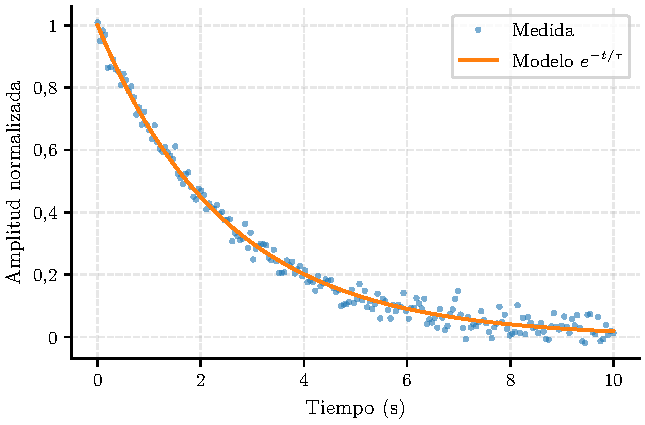
\includegraphics[width=0.7\linewidth]{generadas/ejemplo_curva}
%     \captionof{figure}{Descripción breve.}
%   \end{center}
\begin{resumenproyecto}{RESUMEN DEL PROYECTO}

\apartadoresumen{1. Introducción}
Contexto del problema, motivación y objetivos del trabajo en pocas líneas.

\apartadoresumen{2. Metodología}
Qué se ha hecho y cómo: enfoque, herramientas y decisiones principales.

\apartadoresumen{3. Resultados}
Resultados cuantitativos más relevantes. Usa cifras concretas, por
ejemplo un error del \qty{3.9}{\percent} frente al \qty{6.9}{\percent}
de la referencia.

\apartadoresumen{4. Conclusiones}
Qué se concluye y qué queda abierto.

\vspace{1em}
\noindent\textbf{Palabras clave:} \PalabrasClave

\end{resumenproyecto}

% !TeX root = ../main.tex
% ABSTRACT: traducción del resumen. Se compone en inglés (guiones,
% comillas) y con punto decimal, también en \num y \qty de siunitx.
\begin{resumenproyecto}{ABSTRACT}
\begin{otherlanguage}{english}
\sisetup{output-decimal-marker={.}}

\apartadoresumen{1. Introduction}
Problem context, motivation and objectives.

\apartadoresumen{2. Methodology}
What was done and how.

\apartadoresumen{3. Results}
Key quantitative results, e.g.\ an error of \qty{3.9}{\percent}.

\apartadoresumen{4. Conclusions}
Main conclusions and open lines of work.

\vspace{1em}
\noindent\textbf{Keywords:} \Keywords

\end{otherlanguage}
\end{resumenproyecto}


\cleardoublepage
\tableofcontents
\listoffigures
\listoftables
\lstlistoflistings
% !TeX root = ../main.tex
% Lista de acrónimos (paquete acronym). En el texto:
%   \ac{ODS}   -> primera vez "Objetivos de Desarrollo Sostenible (ODS)", luego "ODS"
%   \acs{ODS}  -> siempre la sigla     \acl{ODS} -> siempre el nombre largo
%   \acp{...}  -> plural (añade una "s"; si el plural es irregular usa \acs)
% En títulos y pies de figura escribe la sigla como texto normal: si usas
% \ac o \acs, la "primera aparición" ocurre en el índice.
% Mantén la lista en orden alfabético. El argumento opcional de
% \begin{acronym} es la sigla más larga (para alinear la columna).
\cleardoublepage
\chapter*{Lista de acrónimos}
\addcontentsline{toc}{chapter}{Lista de acrónimos}
\begin{acronym}[ODS]
  \acro{CI}{integración continua (\textit{Continuous Integration})}
  \acro{ODS}{Objetivos de Desarrollo Sostenible}
  \acro{SI}{Sistema Internacional de Unidades}
  \acro{TFG}{Trabajo Fin de Grado}
  \acro{TFM}{Trabajo Fin de Máster}
\end{acronym}


% ---------------------------------------------------------------------
%  CUERPO
% ---------------------------------------------------------------------
\mainmatter
\pagestyle{fancy}

% !TeX root = ../main.tex
\chapter{Introducción}\label{cap:introduccion}

\section{Contexto y motivación}\label{sec:motivacion}

Presenta el problema, por qué es relevante y a quién afecta. Termina con
una o dos frases que expliquen qué aporta este trabajo.

Los acrónimos se escriben con \verb|\ac{...}|: la primera aparición de
\ac{ODS} se expande y las siguientes (\ac{ODS}) no.

\section{Objetivos}\label{sec:objetivos}

El objetivo general de este \ac{TFG} es \pendiente{redactar el objetivo general}.

Los objetivos específicos son:
\begin{enumerate}
  \item \textbf{O1.} Objetivo medible y verificable.
  \item \textbf{O2.} \ldots
  \item \textbf{O3.} \ldots
\end{enumerate}
El \cref{cap:conclusiones} revisa el grado de cumplimiento de cada uno.

\section{Metodología y planificación}\label{sec:planificacion}

Describe cómo se ha organizado el trabajo. El diagrama de la
\cref{fig:gantt} debe coincidir con los hitos (\textit{milestones}) del
tablero del proyecto en GitHub.

\begin{figure}[H]
  \centering
  \begin{ganttchart}[
      hgrid, vgrid={*1{draw=black!10}},
      x unit=0.3cm, y unit chart=0.6cm,
      title label font=\tiny,
      bar label font=\small,
      milestone label font=\small\itshape,
      bar/.append style={fill=blue!30},
    ]{1}{36}
    \gantttitle{Semanas}{36} \\
    \gantttitlelist{1,...,36}{1} \\
    \ganttbar{Arranque y propuesta}{1}{2} \\
    \ganttbar{Estado del arte}{2}{9} \\
    \ganttbar{Planteamiento}{6}{10} \\
    \ganttbar{Desarrollo}{9}{20} \\
    \ganttmilestone{Seguimiento}{15} \\
    \ganttbar{Resultados}{18}{25} \\
    \ganttbar{Redacción final}{22}{29} \\
    \ganttbar{Revisión y entrega}{29}{33} \\
    \ganttmilestone{Defensa}{36}
  \end{ganttchart}
  \caption{Planificación temporal del trabajo.}
  \label{fig:gantt}
\end{figure}

\section{Alineación con los Objetivos de Desarrollo Sostenible}\label{sec:ods}

Resume en un párrafo con qué \acs{ODS} se relaciona el trabajo. El
análisis detallado va en el \cref{anx:ods}.

\section{Estructura de la memoria}\label{sec:estructura}

El \cref{cap:estado-arte} revisa el estado del arte. El
\cref{cap:planteamiento} plantea el problema y la solución propuesta. El
\cref{cap:desarrollo} describe el desarrollo y el \cref{cap:resultados}
presenta los resultados. Por último, el \cref{cap:conclusiones} recoge las
conclusiones y las líneas de trabajo futuro.

% !TeX root = ../main.tex
\chapter{Estado del arte}\label{cap:estado-arte}

Revisa críticamente lo que ya existe: no basta con enumerar trabajos,
hay que compararlos y detectar el hueco que cubre este proyecto. Frase añadida para probar la CI.

\section{Cómo citar}

Las referencias se guardan en \texttt{bibliografia/referencias.bib} y se
citan con \verb|\cite{clave}|: por ejemplo, la tipografía de este documento
se basa en \TeX{}~\cite{Knuth1984TeXbook} y \LaTeX{}~\cite{Lamport1994LaTeX}.
Se pueden citar varias a la vez~\cite{Knuth1984TeXbook, Lamport1994LaTeX}.
Usa claves del tipo \texttt{AutorAñoTema} e incluye siempre el DOI cuando
exista.

\section{Comparativa}

Una tabla comparativa suele ser la forma más clara de cerrar el capítulo
(\cref{tab:comparativa}).

\begin{table}[H]
  \centering
  \caption{Comparativa de soluciones existentes.}
  \label{tab:comparativa}
  \begin{tabular}{lccc}
    \toprule
    Solución & Coste & Precisión & Disponibilidad \\
    \midrule
    Alternativa A & Alto  & Alta  & Comercial \\
    Alternativa B & Bajo  & Media & Abierta   \\
    \textbf{Este trabajo} & \textbf{Bajo} & \textbf{Alta} & \textbf{Abierta} \\
    \bottomrule
  \end{tabular}
\end{table}

\section{Posicionamiento del trabajo}

Explica qué aporta este trabajo respecto a lo revisado.

% !TeX root = ../main.tex
\chapter{Planteamiento del problema}\label{cap:planteamiento}

Define con precisión el problema, los requisitos y la solución propuesta
a alto nivel, antes de entrar en detalles de implementación.

\section{Requisitos}

\begin{table}[H]
  \centering
  \caption{Requisitos del sistema.}
  \label{tab:requisitos}
  \begin{tabularx}{\linewidth}{llX}
    \toprule
    ID & Tipo & Descripción \\
    \midrule
    R1 & Funcional    & El sistema debe \ldots \\
    R2 & No funcional & El tiempo de respuesta debe ser inferior a \qty{10}{\milli\second}. \\
    \bottomrule
  \end{tabularx}
\end{table}

\section{Arquitectura propuesta}

Los diagramas de bloques sencillos se pueden dibujar directamente con
TikZ (\cref{fig:arquitectura}), de modo que el texto de la figura use la
misma tipografía que la memoria.

\begin{figure}[H]
  \centering
  \begin{tikzpicture}[
      node distance=1.8cm,
      bloque/.style={draw, rounded corners, minimum width=2.6cm,
                     minimum height=1cm, fill=blue!8, align=center},
      flecha/.style={-Stealth, thick}]
    \node[bloque] (entrada) {Adquisición};
    \node[bloque, right=of entrada] (proceso) {Procesado};
    \node[bloque, right=of proceso] (salida) {Visualización};
    \draw[flecha] (entrada) -- node[above]{\small datos} (proceso);
    \draw[flecha] (proceso) -- node[above]{\small resultados} (salida);
  \end{tikzpicture}
  \caption{Arquitectura general de la solución.}
  \label{fig:arquitectura}
\end{figure}

\section{Modelo matemático}

Las ecuaciones se numeran y referencian igual que las figuras
(\cref{ec:modelo}):
\begin{equation}
  \label{ec:modelo}
  y(t) = y_0 \, e^{-t/\tau} + \int_0^t h(t-s)\, u(s) \dif s
\end{equation}
donde $\tau = \qty{2.5}{\second}$ es la constante de tiempo.

% !TeX root = ../main.tex
% Este capítulo se puede dividir en varios (diseño hardware, software,
% modelo…). Crea un fichero por capítulo y añádelo con \include en main.tex.
\chapter{Desarrollo}\label{cap:desarrollo}

Describe la implementación con el detalle suficiente para que otra
persona pueda reproducirla, y justifica las decisiones de diseño.

\section{Algoritmos}

\begin{algorithm}[H]
  \caption{Media móvil exponencial.}
  \label{alg:ema}
  \KwIn{señal $x_1,\dots,x_N$, factor $\alpha \in (0,1]$}
  \KwOut{señal filtrada $y_1,\dots,y_N$}
  $y_1 \gets x_1$\;
  \For{$k \gets 2$ \KwTo $N$}{
    $y_k \gets \alpha x_k + (1-\alpha)\, y_{k-1}$\;
  }
  \Return{$y$}
\end{algorithm}

\section{Código}

Incluye solo los fragmentos imprescindibles (\cref{lst:ema}). El código
completo debe estar en el repositorio y se referencia desde el
\cref{anx:codigo}.

\begin{lstlisting}[language=Python, caption={Implementación del \cref{alg:ema}.}, label={lst:ema}]
def ema(x, alpha):
    """Media móvil exponencial."""
    y = [x[0]]
    for xk in x[1:]:
        y.append(alpha * xk + (1 - alpha) * y[-1])
    return y
\end{lstlisting}

% !TeX root = ../main.tex
\chapter{Resultados}\label{cap:resultados}

Empieza describiendo el protocolo experimental (datos, métricas,
semillas…) para que los resultados sean reproducibles.

\section{Protocolo experimental}

\section{Resultados principales}

Las figuras con datos se generan con los scripts de
\texttt{scripts/figuras/} (\cref{fig:ejemplo}): nunca a mano ni como
capturas de pantalla. Así usan la misma tipografía que la memoria, llevan
coma decimal y se pueden regenerar si cambian los datos.

\begin{figure}[H]
  \centering
  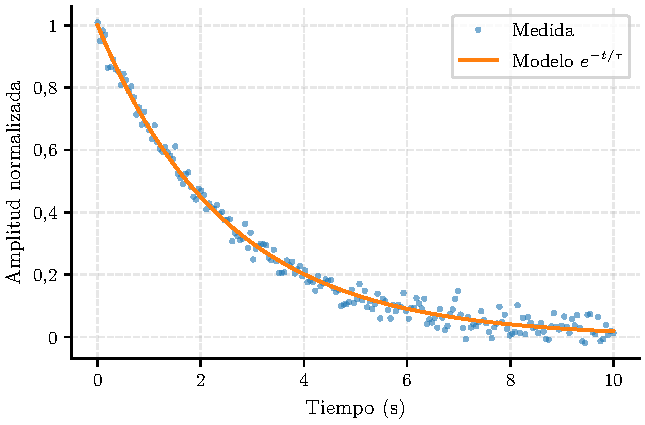
\includegraphics[width=0.8\linewidth]{generadas/ejemplo_curva}
  \caption{Figura de ejemplo generada con \texttt{scripts/figuras/ejemplo\_curva.py}.}
  \label{fig:ejemplo}
\end{figure}

Las tablas de resultados también pueden generarse desde el código
(\cref{tab:ejemplo}), lo que evita errores al copiar cifras a mano.

% Generado automáticamente por scripts/figuras. NO EDITAR A MANO.
\begin{table}[H]
  \centering
  \caption{Métricas de error del ejemplo (generada desde Python).}
  \label{tab:ejemplo}
  \begin{tabular}{lc}
    \toprule
    Métrica & Valor \\
    \midrule
    MAE & \num{0.021} \\
    RMSE & \num{0.026} \\
    Error máximo & \num{0.087} \\
    $\tau$ (s) & \num{2.500} \\
    \bottomrule
  \end{tabular}
\end{table}


\section{Discusión}

Interpreta los resultados: qué significan, por qué salen así y qué
limitaciones tienen.

% !TeX root = ../main.tex
\chapter{Conclusiones y trabajo futuro}\label{cap:conclusiones}

\section{Conclusiones}

\section{Cumplimiento de los objetivos}

\begin{table}[H]
  \centering
  \caption{Grado de cumplimiento de los objetivos planteados en la \cref{sec:objetivos}.}
  \label{tab:cumplimiento}
  \begin{tabularx}{\linewidth}{lXl}
    \toprule
    Objetivo & Evidencia & Estado \\
    \midrule
    O1 & \cref{sec:objetivos} & Cumplido \\
    O2 & \ldots & Parcial \\
    \bottomrule
  \end{tabularx}
\end{table}

\section{Líneas de trabajo futuro}


% ---------------------------------------------------------------------
%  BIBLIOGRAFÍA Y ANEXOS
% ---------------------------------------------------------------------
\cleardoublepage
\printbibliography[heading=bibintoc]

\begin{appendices}
% !TeX root = ../main.tex
\chapter{Presupuesto}\label{anx:presupuesto}

El presupuesto se desglosa en materiales, herramientas (amortización) y
personal. Los importes se escriben con \verb|\qty{}{\euro}| o \verb|\EUR{}|
para que el formato sea uniforme.

\begin{table}[H]
  \centering
  \caption{Presupuesto total del proyecto.}
  \label{tab:presupuesto}
  \begin{tabular}{lS[table-format=5.2]}
    \toprule
    Concepto & {Importe (\euro)} \\
    \midrule
    Materiales                 &   350.00 \\
    Herramientas (amortización) &   120.00 \\
    Personal (\qty{300}{\hour} a \qty{30}{\euro\per\hour}) & 9000.00 \\
    \midrule
    Subtotal                   &  9470.00 \\
    IVA (\qty{21}{\percent})   &  1988.70 \\
    \midrule
    \textbf{Total}             & 11458.70 \\
    \bottomrule
  \end{tabular}
\end{table}

% !TeX root = ../main.tex
\chapter{Alineación con los Objetivos de Desarrollo Sostenible}\label{anx:ods}

Explica, para cada \ac{ODS} relevante, de qué forma contribuye el trabajo.
Sé concreto: menciona la meta (p.~ej.\ 7.3) y el mecanismo.

\section*{ODS 7: Energía asequible y no contaminante}

\section*{ODS 9: Industria, innovación e infraestructura}

\begin{table}[H]
  \centering
  \caption{Resumen de la contribución a los ODS.}
  \label{tab:ods}
  \begin{tabularx}{\linewidth}{llX}
    \toprule
    ODS & Meta & Contribución \\
    \midrule
    7 & 7.3 & \ldots \\
    9 & 9.4 & \ldots \\
    \bottomrule
  \end{tabularx}
\end{table}

% !TeX root = ../main.tex
\chapter{Código y reproducibilidad}\label{anx:codigo}

Indica dónde está el código (repositorio y versión etiquetada), cómo se
instala y cómo se reproducen los resultados del \cref{cap:resultados}:
versiones, datos (con su DOI), semillas y comandos exactos.

\begin{lstlisting}[language=bash, caption={Reproducción de las figuras de la memoria.}, label={lst:reproducir}]
python3 -m venv .venv && source .venv/bin/activate
pip install -r scripts/requirements.txt
make figuras
make memoria
\end{lstlisting}

\end{appendices}

\end{document}
